\documentclass[border=20pt,tikz]{standalone}
\usepackage{amsfonts}
\usepackage{amsmath}
\usepackage{wasysym}
\usepackage{amssymb}
\usepackage{physics}
\usepackage{tikz}
\usepackage{bm}
\usepackage[outline]{contour} % glow around text
\usetikzlibrary{calc}
\usetikzlibrary{angles,quotes} % for pic
\usetikzlibrary{arrows.meta}
\usetikzlibrary{patterns}
\tikzset{>=latex} % for LaTeX arrow head
\contourlength{1.35pt}

\colorlet{xcol}{blue!70!black}
\colorlet{vcol}{green!60!black}
\colorlet{myred}{red!65!black}
\colorlet{mydarkred}{red!40!black}
\colorlet{mypurple}{blue!60!red!80}
\colorlet{mydarkgreen}{green!20!black}
\colorlet{acol}{red!50!blue!80!black!80}
\tikzstyle{rvec}=[->,xcol,very thick,line cap=round]
\tikzstyle{vvec}=[->,vcol,very thick,line cap=round]
\tikzstyle{myarr}=[{Latex[length=3,width=3]}-,xcol]
\tikzstyle{myarr2}=[{Latex[length=2,width=2.5]}-{Latex[length=2,width=2.5]}]
\tikzstyle{force}=[->,myred,very thick,line cap=round]
\tikzstyle{Fproj}=[force,myred!40]
\tikzstyle{CM}=[mydarkred,fill=red!80!black!80]


\tikzstyle{mass}=[line width=0.6,draw=red!30!black, %rounded corners=1,
                  top color=mydarkred!30,bottom color=mydarkred!10,shading angle=30]

\tikzstyle{mass2}=[line width=0.4,draw=black, %rounded corners=1,
                  top color=black!40,bottom color=black!40]
                  
\tikzstyle{dark mass}=[line width=0.3,red!30!black, %rounded corners=1,
                       top color=mydarkred!40,bottom color=mydarkred!60,shading angle=30]
\tikzstyle{ground}=[preaction={fill,top color=black!10,bottom color=black!5,shading angle=20},
                    fill,pattern=north east lines,draw=none,minimum width=0.3,minimum height=0.6]
\tikzstyle{metal}=[fill,top color=black!40,bottom color=black!20,shading angle=10]
\tikzstyle{pulcol}=[draw=blue!30!black,%fill=blue!40!black!10
                    top color=blue!40!black!20,bottom color=blue!40!black!10,shading angle=20]
\tikzstyle{rope}=[brown!70!black,very thick,line cap=round]
\def\rope#1{ \draw[black,line width=1.5] #1; \draw[rope] #1; }
\tikzstyle{mount}=[blue!20!black,fill,top color=blue!20!black!70,bottom color=blue!20!black!40,shading angle=10]

\def\r{0.05} % pulley small radius
\tikzset{
  pics/Tin/.style={
    code={
      \def\R{0.12}
      \draw[pic actions,line width=0.6,#1,fill=white] % ,thick
        (0,0) circle (\R) (-135:.75*\R) -- (45:.75*\R) (-45:.75*\R) -- (135:.75*\R);
  }},
  pics/Tout/.style={
    code={
      \def\R{0.12}
      \draw[pic actions,line width=0.6,#1,fill=white] (0,0) circle (\R);
      \fill[pic actions,#1] (0,0) circle (0.3*\R);
  }},
  pics/rotarr/.style={
    code={
      \draw[white,very thick] ({#1*cos(200)},0) arc(-200:30:{#1} and {#1/2}) --++ (125:0.1);
      \draw[->,mydarkgreen] ({#1*cos(200)},0) coordinate (W1) arc(-200:20:{#1} and {#1/2}) node[midway] (W2) {} --++ (125:0.1) coordinate (W3);
  }},
  pics/pulley/.style={
    code={
      \draw[pulcol,line width=0.6] (0,0) circle (#1);
      \draw[pulcol,thick] (0,0) circle (\r);
  }},
  pics/mount/.style args={#1:#2}{ % angle, length
    code={
      \draw [mount] (0,0)++(#1-90:0.9*\r) arc (#1-90:#1-270:0.9*\r) --++ (#1:#2) --++ (#1-90:1.8*\r) -- cycle;
    }
  },
  pics/Tin/.default=mypurple,
  pics/Tout/.default=mypurple,
  pics/rotarr/.default=0.4,
  pics/pulley/.default=0.3,
}


\newcommand\rightAngle[4]{
  \pgfmathanglebetweenpoints{\pgfpointanchor{#2}{center}}{\pgfpointanchor{#3}{center}}
  \coordinate (tmpRA) at ($(#2)+(\pgfmathresult+45:#4)$);
  \draw[white,line width=0.7] ($(#2)!(tmpRA)!(#1)$) -- (tmpRA) -- ($(#2)!(tmpRA)!(#3)$);
  \draw[xcol!30!black] ($(#2)!(tmpRA)!(#1)$) -- (tmpRA) -- ($(#2)!(tmpRA)!(#3)$);
}

\begin{document}


% MOMENT OF INERTIA - DISK
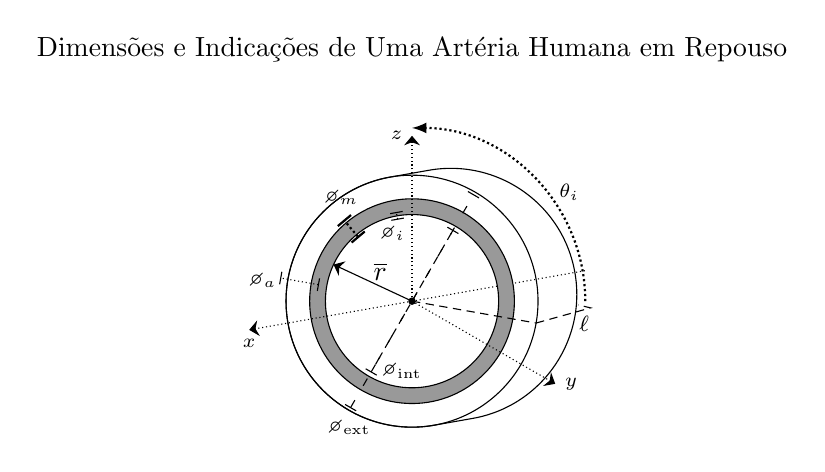
\begin{tikzpicture}[arr/.style={-{Stealth[length=1.2mm, width=2mm]}}]

  \def\R{1.6}
  \def\r{1.1}
  \def\dr{0.2}
  \def\t{0.50} % disk thickness
  \def\angp{10} % perspective
  \def\angdr{60}
  \coordinate (O) at (0,0);
  \coordinate (R) at (50:\r);
  \coordinate (DR1) at (\angdr:\r);
  \coordinate (DR2) at (\angdr:\r+\dr);
  \coordinate (TOP) at (90:\R);
  \coordinate (DOWN) at (270:\R);
  \coordinate (RADIUS) at (155:\R);
  \draw[densely dotted] (0,0) --++ (\angp:1.4*\R);
  \draw[fill=none]
    (\angp+90:\R) --++ (\angp:\t) arc(\angp+90:\angp-90:\R) --++ (\angp-180:\t) arc(\angp-90:\angp-270:\R);
  \draw[fill=none]
    (O) circle(\R);
  \draw[mass2,even odd rule]
    (O) circle(\r+\dr) circle(\r);


    
  \draw[arr] (O) -- (155:\r);
  \node at (137:\r*0.5) [black] {$\overline {r}$}; %,fill=mydarkred!13,inner sep=1
  \draw[densely dotted, arr] (O) -- (-30:\R+0.5) node[right]{\scriptsize $y$}; %,fill=mydarkred!13,inner sep=1
  \draw[densely dotted, arr] (O) -- (90:\R+0.5) node[above, left] {\scriptsize $z$};
  \draw[densely dotted, arr] (0,0) -- (\angp-180:1.5*\R-0.3) node[left, below] {\scriptsize $x$};

  % unitary vectors 
  %\draw[->, gray!90!black!100, thick] (O) -- (\angp-180:0.5) node[midway, above] {\footnotesize $\vb{ \hat i}$}; %,fill=mydarkred!13,inner sep=1

  %\draw[->, gray!90!black!100, thick] (O) -- (-30:0.5) node[left, below]{\footnotesize $\vb{\hat j}$}; %,fill=mydarkred!13,inner sep=1

  %\draw[gray!90!black!100, ->, thick] (O) -- (90:0.5) node[above=-1, right] {\footnotesize $\vb{\hat k}$};

  %dimensions

  \draw[dashed, densely dashed] (O) -- (-10:\R);
  \draw[black, densely dashed] (-10:\R) --++ (0.50,0,-0.5) --++ (-0.2,0,-0.1) node[midway, below] {\footnotesize $\ell$}; 

  \draw[black, thick,|-|, densely dotted] (130:1.05) -- (130:1.35);
  \node at (-0.9,1.1) [black, above] {\scriptsize $\diameter_{m}$};

   \draw[black,|-|, densely dotted] (100:1.05) -- (100:1.15);
  \node at (-0.25,0.65) [black, above] {\scriptsize $\diameter_{i}$};

  \draw[black,|-|, densely dotted] (170:1.20) -- (170:1.7);
  \node at (-1.9,0.05) [black, above] {\scriptsize $\diameter_{a}$};

  \draw[|-|,densely dashed] (240:\r*0.95) -- (60:\r*0.95);
  \node at (-0.13,-1.1) [black, above] {\scriptsize $\diameter_{\mathrm{int}}$};

  \draw[|-|,loosely dashed, thin] (240:\R*0.98) -- (60:\R*0.98);
  \node at (-0.8,-1.82) [black, above] {\scriptsize $\diameter_{\mathrm{ext}}$};

% angle 
    \coordinate (LEFT) at (180:\R);
    \coordinate (RIGHT) at (360:\R);
    
   \pic[draw, thick, ->, angle radius=2.2cm, densely dotted] {angle = RIGHT--O--TOP};
   \node at (30:\R*1.44) [black, above] {\scriptsize $\theta_i$};

   \draw[fill=black] (O) circle (0.04cm);

   \node at (90:\R*2) [black] {Dimensões e Indicações de Uma Artéria Humana em Repouso}; 
\end{tikzpicture}









\end{document}